\begin{figure}[h]
\centering
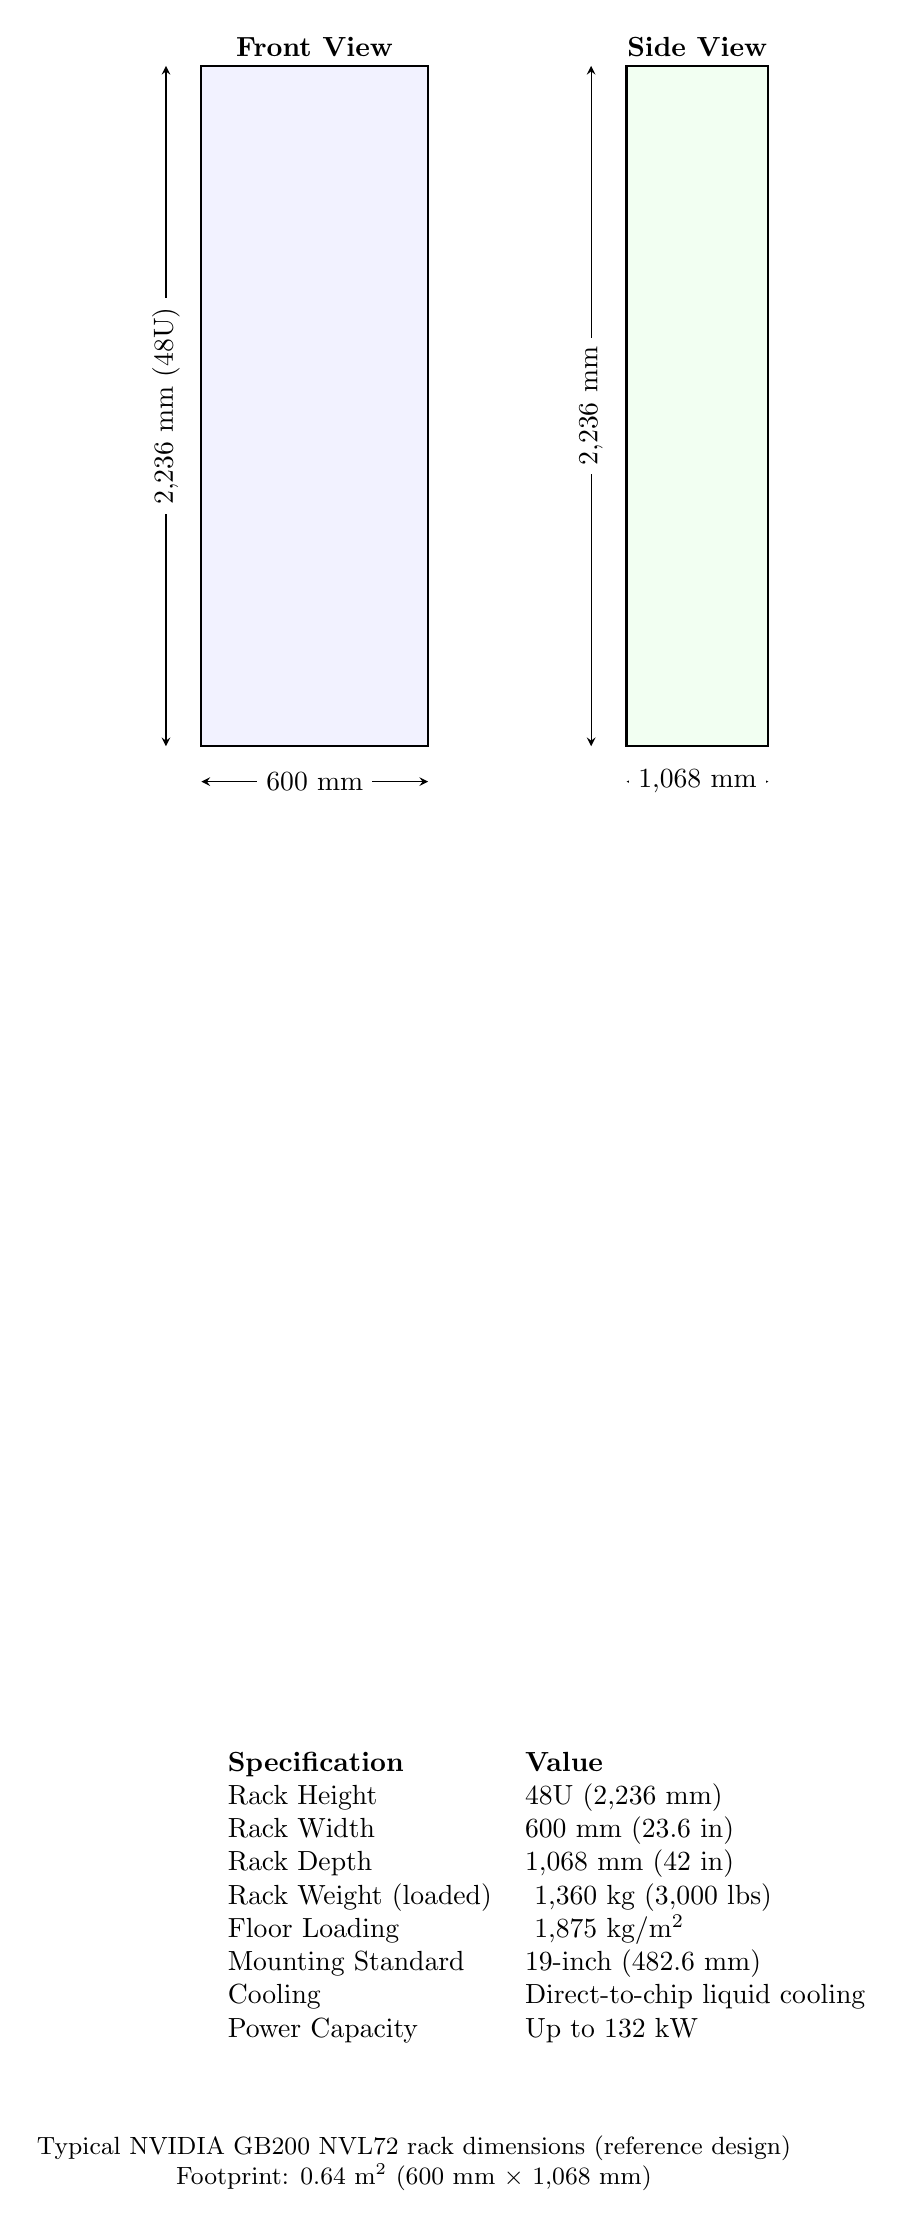
\begin{tikzpicture}[scale=0.9]
% Rack dimensions diagram
\def\rackWidth{4}
\def\rackDepth{2.5}
\def\rackHeight{12}
\def\unitScale{0.8}

% Rack outline (front view)
\draw[thick, fill=blue!5] (0,0) rectangle (\rackWidth*\unitScale, \rackHeight*\unitScale);
\node[above] at (\rackWidth*\unitScale/2, \rackHeight*\unitScale) {\textbf{Front View}};

% Rack dimensions labels
\draw[<->, >=stealth] (0, -0.5) -- node[fill=white] {600 mm} (\rackWidth*\unitScale, -0.5);
\draw[<->, >=stealth] (-0.5, 0) -- node[fill=white, rotate=90] {2,236 mm (48U)} (-0.5, \rackHeight*\unitScale);

% Side view
\begin{scope}[xshift=6cm]
\draw[thick, fill=green!5] (0,0) rectangle (\rackDepth*\unitScale, \rackHeight*\unitScale);
\node[above] at (\rackDepth*\unitScale/2, \rackHeight*\unitScale) {\textbf{Side View}};

\draw[<->, >=stealth] (0, -0.5) -- node[fill=white] {1,068 mm} (\rackDepth*\unitScale, -0.5);
\draw[<->, >=stealth] (-0.5, 0) -- node[fill=white, rotate=90] {2,236 mm} (-0.5, \rackHeight*\unitScale);
\end{scope}

% Table of specifications
\begin{scope}[yshift=-14cm]
\draw (0,0) node[anchor=north west] {
\begin{tabular}{ll}
\toprule
\textbf{Specification} & \textbf{Value} \\
\midrule
Rack Height & 48U (2,236 mm) \\
Rack Width & 600 mm (23.6 in) \\
Rack Depth & 1,068 mm (42 in) \\
Rack Weight (loaded) & ~1,360 kg (3,000 lbs) \\
Floor Loading & ~1,875 kg/m$^2$ \\
Mounting Standard & 19-inch (482.6 mm) \\
Cooling & Direct-to-chip liquid cooling \\
Power Capacity & Up to 132 kW \\
\bottomrule
\end{tabular}
};
\end{scope}

% Notes
\begin{scope}[yshift=-20cm]
\node[align=center, font=\small] at (3,0) {
Typical NVIDIA GB200 NVL72 rack dimensions (reference design)\\
Footprint: 0.64 m$^2$ (600 mm $\times$ 1,068 mm)
};
\end{scope}
\end{tikzpicture}
\caption{Computer rack dimensions for 800 VDC AI infrastructure (NVIDIA GB200 NVL72 reference). High-density racks require reinforced floors and liquid cooling integration.}
\label{fig:rack-dimensions}
\end{figure}
